\section{Discussion} \label{sec:discussion}

% TODO: Why is conv-char-NN so much better than conv-char-word-NN?
% TODO: Discuss how the system should be used.

In this section we will discuss the results of our experiments, our expectations
compared to the actual performance, the applicability of the methods we
implemented in the real world and we will present the kind of feedback we are
able to give to teachers of why our networks make certain decisions.


\subsection{Results}

We presented our results in Section \ref{sec:results}. We did not succeed in
achieving an accusation error of less than 10\% while catching 95\% of cheaters.
However, we believe that some of the methods show promising results. While
all the networks we applied to the test dataset beat our baselines the best
performing network was the \gls{conv-char-NN}. This network had an accusation
error closest to the one required in addition to having the highest overall
accuracy in all the categories we tested it on. It was closely followed by
network \gls{conv-char-word-NN}. The \gls{rec-sent-NN} had sub-par performance.
It is however worth noting that this could very well be due to the infeasibility
of running any of our \glspl{RNN} on the character or word level of the texts
supplied to it. We hypothesize that the accuracy of an RNN would be greatly
increased had it been run on a lower linguistic level. In experiments we found
that \glspl{CNN} also performed badly on the sentence level in our use case.
Unfortunately we were not able to train an \gls{RNN} on one of the lower
linguistic levels due to computational constraints.

Comparing our validation dataset results from Table
\ref{tab:experiment-validation-results} to our test results we can clearly see a
difference. The results from the validation dataset meets the requirements for
the accusation error, while the test results does not. However, this difference
is justified as it was on the validation set that we found the prediction system
and threshold that got us under said requirement. Therefore it stands to reason
that the models would have a somewhat lower performance when applied to a fresh,
untouched test dataset. This lowered performance takes form of an increased
accusation error, and a decreased accuracy. This is the case for machine
learning tasks in general.

It is worth noting that the number of false accusations on the validation
dataset were very small. It seems like we have overfitted a lot on the
validation dataset and found the exact point before many false accusations were
made. We should have maybe used a slightly lower threshold such that we would
not have achieved such a high accusation error on the test dataset.


\subsubsection{AUROC}

A more general description of a model's performance can be computed using the
\gls{AUC} of the \gls{ROC}-curve of a model better known as \gls{AUROC}.
A \gls{ROC} curve is the \gls{FPR} plotted against the \gls{TPR} both of
which are defined in Section \ref{sec:method}. \gls{AUROC} is a measure of
discrimination, or a measure of the amount of certainty our model has when it
makes a decision.

The ROC curves and AUROC results for the different networks we produced can be
seen in Figure \ref{fig:AUROC}. These figures reinforce the relationship between
the networks already expressed. The \gls{conv-char-NN} still performed best.
It was however very closely followed by the \gls{conv-char-word-NN}. At some
points the two \gls{ROC}-curves overlap when using the dataset with 4\% negative
samples and with the constrained configuration.

While the \gls{rec-sent-NN} does have the worst AUROC score it is higher
than we anticipated when looking back at the results presented in Section
\ref{sec:results}. This might be attributed to the model working well generally
but not adapting very well to thresholding compared to the other two networks.

\begin{figure}
    \centering
    \begin{minipage}{.8\textwidth}
        \centering
        \textbf{Constrained ROC-Curve and AUROC for each network}
        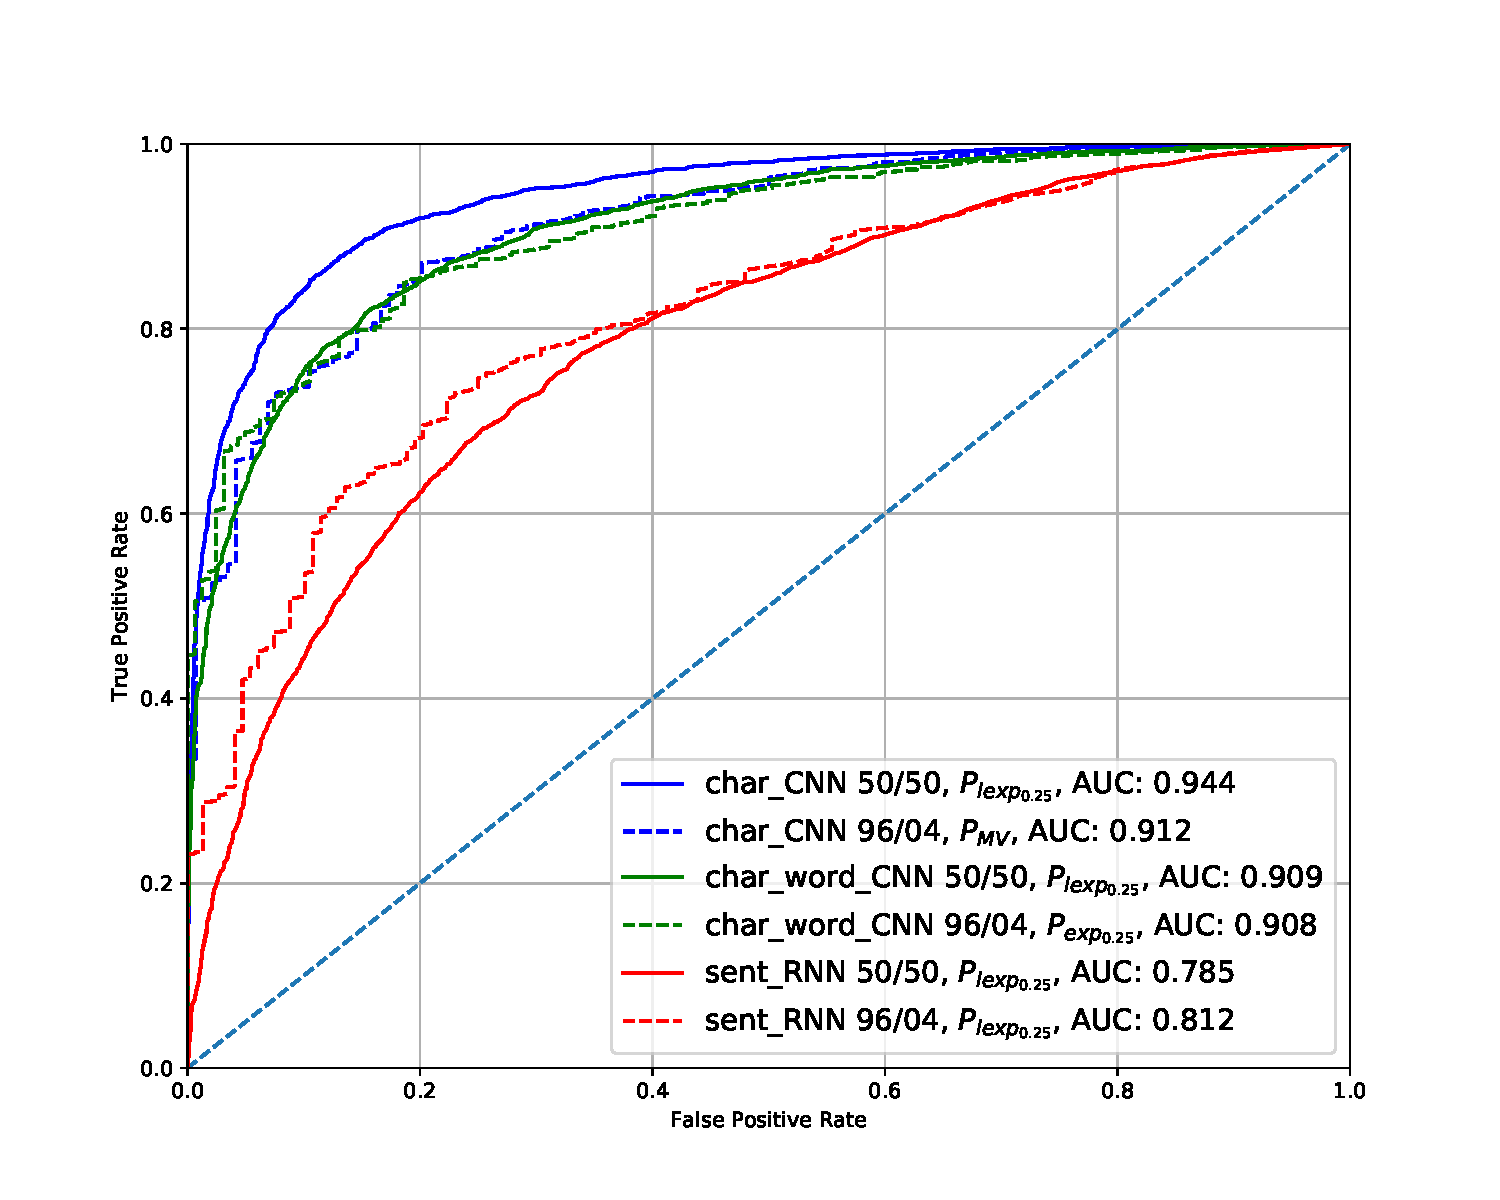
\includegraphics[width=1\linewidth]{./pictures/discussion/AUROC_Constrained}
    \end{minipage}\\
    \begin{minipage}{.8\textwidth}
        \centering
        \textbf{Unconstrained ROC-Curve and AUROC for each network}
        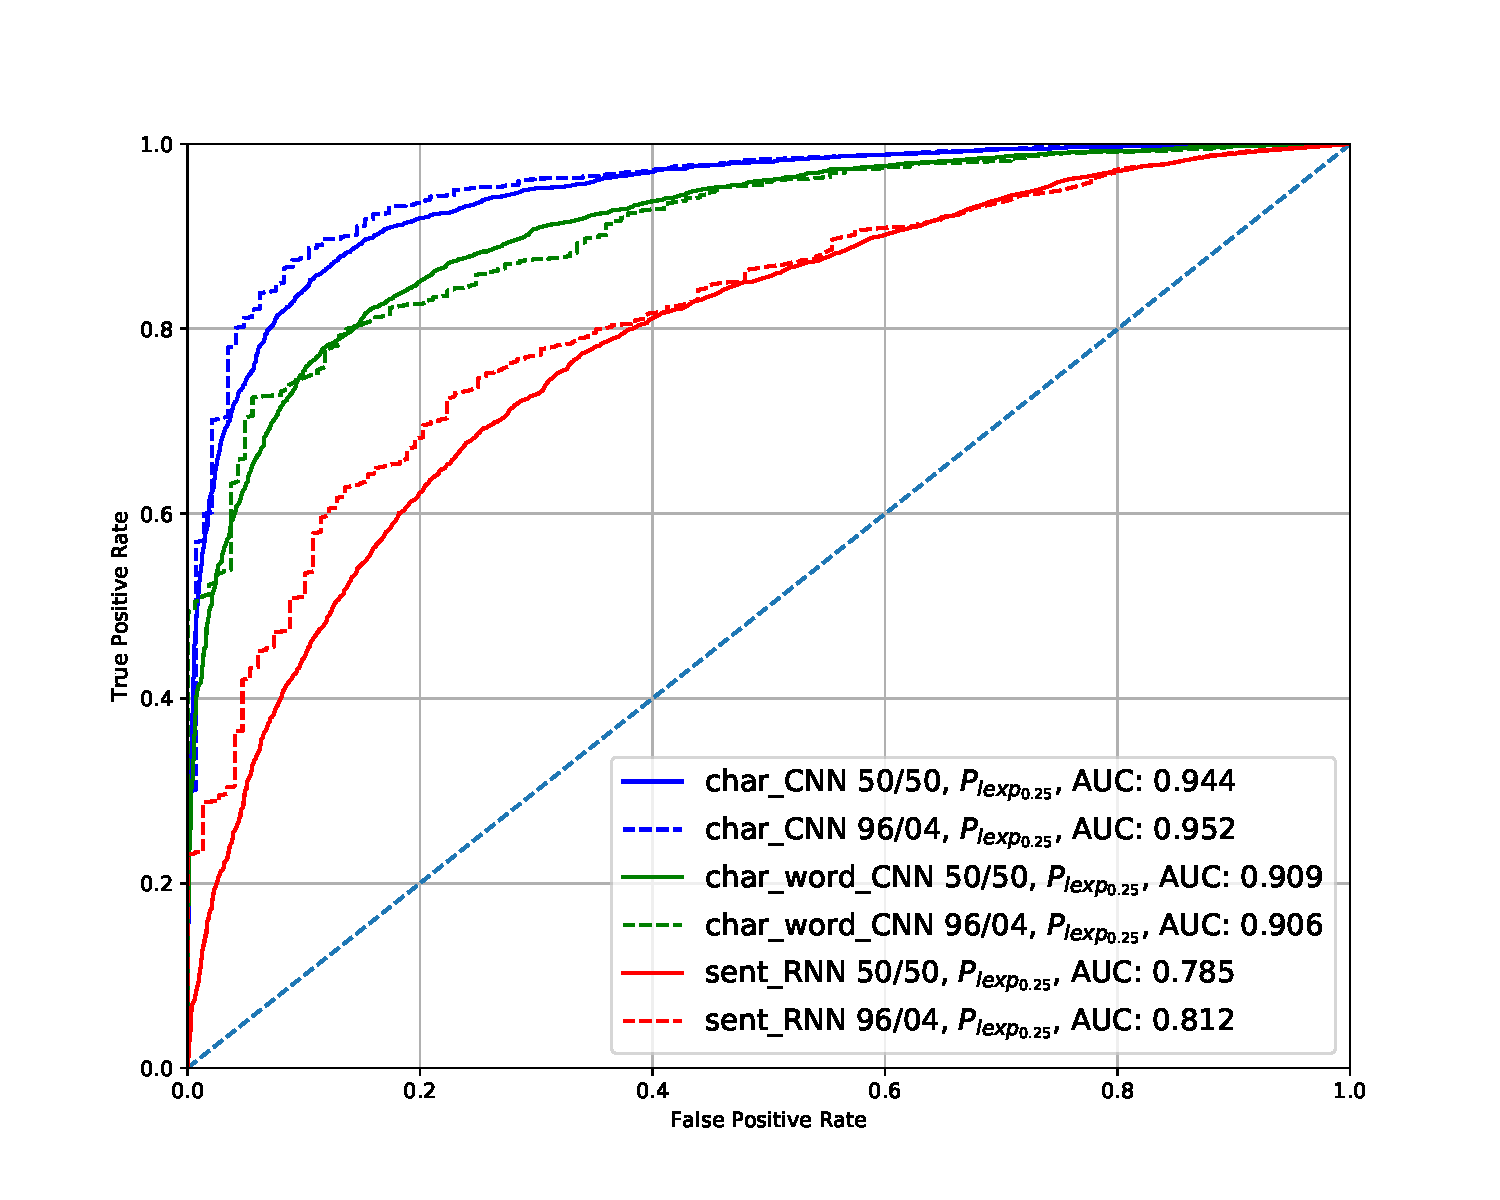
\includegraphics[width=1\linewidth]{./pictures/discussion/AUROC_Unconstrained}
    \end{minipage}
    \caption{The \gls{ROC}-curve for the three networks produced plotted for
        both of the possible data sample splits. We used the configuration of
        threshold and prediction system that produced the best results on the
        validation dataset \gls{C}.}
    \label{fig:AUROC}
\end{figure}

Our \gls{AUROC} scores are generally very good. We can see in the figures that
as expected the score on the 50\% negative dataset is about the same as on the
4\% negative dataset. Our reported results (not \gls{AUROC} score) looks much
worse on the 4\% dataset but it is also much harder to achieve a good results on
a dataset with such few negatives. The \gls{AUROC} scores show that we retain a
good discriminative model even when the dataset changes to match the real world
data.


\subsubsection{Comparison Between Methods}

Comparing our two convolutional networks we see that \gls{conv-char-NN} has the
highest accuracy and lowest accusation error. Recalling that \gls{conv-char-NN}
works on the character level and \gls{conv-char-word-NN} works on both
the character and word level it would seem as if the word level does not
contribute much to the classification. However we have to keep in mind that
\gls{conv-char-NN} generally had more resources available. We used more time
experimenting on that network and it had more dense layers and more convolutions
available. We would have liked to have experimented more with different
linguistic layers. It would have been especially interesting to develop a
network using both the character, word, sentence and \gls{POS} tag level. It
would also have been interesting to create a version of \gls{conv-char-word-NN}
that had as many character level convolutions as \gls{conv-char-NN} and as many
dense layers but then had a separate word level input channel. Then we would
have been able to conclusively determine whether or not a word channel were
worth it in our network architecture.

Comparing our convolutional networks and our recurrent network we see that
the convolutional networks performs much better. We briefly discussed in
Section \ref{subsubsec:siamese_networks} the advantages and disadvantages of
\glspl{CNN} vs \glspl{RNN}. The discussion was based on a comparative study by
\citep{DBLP:journals/corr/0001KYS17}. The conclusions of the study was that both
recurrent and convolutional networks works well for \gls{NLP} but that they
work well for different problem types. If the content of a text is important
for solving a specific problem such as for \textit{Automatic Text Summation}
\glspl{RNN} works best \citep{DBLP:journals/corr/ZengLFU16}. Similarly if the
content is not important such as authorship verification tasks convolutional
networks generally works better \citep{DBLP:journals/corr/0001KYS17}. Our
results back up that finding. We found that it was much easier to develop a
convolutional neural network that worked well in our setting than a recurrent
neural network.


\subsubsection{Previous Work on MaCom Data}

In Section \ref{subsec:previous_work_using_macoms_dataset} we describe other
experiments with authorship attribution and verification on MaCom's dataset.
In this section we compare our authorship verification results with those
earlier results. The first experiment we compare against is \citep{aalykke2016}.
\citet{aalykke2016} evaluated his performance using the sensitivity and
specificity of his best performing configuration. The sensitivity is reported at
95.0\% and the specificity at 71.9\%. Those results were obtained on a dataset
with 500 positive cases and 500 negative cases. \citet{aalykke2016} commented
that his results were not directly comparable to the real world as he used a
dataset with 50\% negative samples. We have focused on developing methods that
work best on a dataset with 4\% negative samples. We have however reported
results when maximizing accuracy on a 50\% negative dataset which is comparable
to his results. In our best configuration on the 50\% negative dataset, we
obtained a sensitivity of 91.0\% and a specificity of 82.1\%. That means that
we had a worse sensitivity but a better specificity. The accuracy obtained by
\citet{aalykke2016} was $\frac{0.95 + 0.719}{2} = 83.5\%$ while our accuracy was
at $86.5\%$, so we had a higher accuracy.

The results produced by \citet{aalykke2016} are impressive considering he only
used the distances between feature sets to compare assignments. One caveat to
consider when looking at his results compared to ours is the fact that he tried
all thresholds on the test dataset and reported the best results obtained.
The results we report used a configuration found on a validation dataset and
evaluated on a test dataset. We can therefore expect that our results will be
an unbiased estimate of real world performance while the best results produced
by \citet{aalykke2016} will probably not. Furthermore \citet{aalykke2016} used
a test dataset that only contained \gls{SRP} assignments. In our test dataset
we predict the newest text in an author's library which is not necessarily the
\gls{SRP} assignment. That gives \citet{aalykke2016} another advantage since
the \gls{SRP} assignments are generally longer assignments and therefore give a
better picture of an author's writing style.

To summarize, \citet{aalykke2016} have a lower accusation error than we do
on 5\% (100\% - 95\%) vs our 9.87\%. At the same time they also have a lower
specificity of 71.9\% vs our 82.1\%. So which method to use is a tradeoff
between how many false accusations to allow vs how large a fraction of cheaters
they want to catch. We believe that our method would have obtained better results if
we had used a test dataset of only \gls{SRP} assignments. For future work,
such a test could be relevant as well as interesting.

We also compare our results with another experiment. This experiment was
described in \citep{hansen2014}. They measured their results using a simple
accuracy. They achieved a maximum accuracy of 84\%. They did not specify the
fraction between negatives and positives that they evaluate against. We assume
that they evaluate on a 50/50 percent split as \citet{aalykke2016}. Again our
most comparable result is when we maximize accuracy on a 50/50 split. Our
best accuracy in that setting were 86.54\%. \citet{hansen2014} focused on the
computation time of their method. Since they used an author specific model they
had to train a separate model on each new author and a new model each time an
author turned in a new assignment. That is where our generalizing model has an
advantage. We only have to train the model once and after that it can be used
on any new author. The prediction time of a neural network is lower than the
training time of an \gls{SVM}.

\citet{hansen2014} found that recent texts were more important than older
texts for predicting an author's writing style. During our experimentation
we came to that same conclusion. Most of the best configurations we found
used a weight function based on the time in which the assignments were
turned in. We will discuss how students writing styles evolve in Section
\ref{subsec:writing_style_changes}.

We seem to have a very comparable but slightly better performance than previous
experiments that made use of MaCom's dataset. Our results are not significantly
better, but we have several advantages over previous methods. We have focused
on performance on a dataset split with 96\% positives and 4\% negatives, and we
have implemented a generalizing model. The data split means that our results are
more reliable as estimates of real world performance, and the generalizing model
means that we save computation time.


\subsubsection{Other Authorship Verification Results}
\label{subsubsec:other_authorship_verification_results}

As described earlier \citet{qian:2018} received excellent authorship
verification results. They achieved an accuracy of 99.8\%. We based our
recurrent network on their architecture as we wanted to replicate their results.
Our recurrent network had nowhere near as high accuracy as we achieved an
accuracy of 68.6\% on the test dataset. We had not suspected our results to be
exactly as good as \citet{qian:2018}, but a drop that big was not expected.
However, there are some important differences between the datasets the networks
are trained and tested on.

The dataset \citet{qian:2018} used were the Reuter\_50\_50 dataset
\\\citep{Dua:2017}. It contains 50 authors each with 100 texts. For each
author 50 of his/her 100 texts were in the training dataset and 50 were in
the testing dataset. Furthermore the texts were all from the same topic
(corporate/industrial). In contrast, our dataset uses completely different
authors between the training and test dataset and we have texts spanning many
topics.

% TODO: Here we should have a graph showing the training before and after
% using different authors.

At one point we trained a network using the \citet{qian:2018} inspired
architecture on a training and validation dataset using the same authors. Here
we observed that the validation accuracy followed the training accuracy far
longer than was the case for a validation dataset containing different authors.
We therefore believe that the reason \citet{qian:2018} obtained such good
results is that the test and training datasets consisted of the same authors. We
wanted to create a generalizing model that were trained once and used many times
which meant that this architecture did not work as well for our purpose.

An interesting area for further research and experimentation could be creating
a combination between our generalizing models and author specific neural
network models. A disadvantage when using author specific models is that it
is necessary to train a different model for each author and retrain models
when new material is turned in by an existing author. However they have the
advantage of often being more accurate than generalizing models. We could have
used our generalizing model to find potential ghostwriting candidates. Using
the \gls{conv-char-word-NN} we could catch 32.6\% of the ghostwriters on a 4\%
negative dataset but we could only do so with an accusation error of 47.7\%. We
could stop taking the output of the generalizing model as the truth, and then
use a author specific network to verify the result of the generalizing model.
Then we would only be required to train a generalized model in the cases where
we suspect ghostwritten assignments.


\subsection{Teacher Feedback}\label{subsec:teacher_feedback_text_comparisons}

As mentioned in Section \ref{sec:introduction} we wanted to explore what kind
of feedback we could give teachers in conjunction with the bare predictions.
As explained earlier the system is not meant to be the final judge of which
students are cheating but is rather meant as a support system for teachers that
are already suspicious of a student. We have focused on the \gls{conv-char-NN}
network since it performed best on the test dataset.


\subsubsection{Extracting Important Features}

Previously we have looked at the output of the feature extraction layer to
obtain information on what a specific network was looking at during the
creation of the networks. We wanted to do something similar for teacher
feedback. Recall that the \gls{conv-char-NN} started with a convolutional
layer followed by a max pool layer. For that reason the larger output
of a convolution is considered the most important one for a particular
sequence. The output of the feature extraction can be thought of as in Figure
\ref{fig:feature_extraction_output_example}. Each filter gives a single output
that is the maximum output of any filter position. The combining function for
the third network is the absolute difference. This means that when we compare
texts $t$ and $t'$, the output of the combination will be high for a particular
filter iff the maximum output of that filter is significantly different for $t$
and $t'$.

\begin{figure}
    \centering
    \textbf{Teacher Feedback Example}\par\medskip
    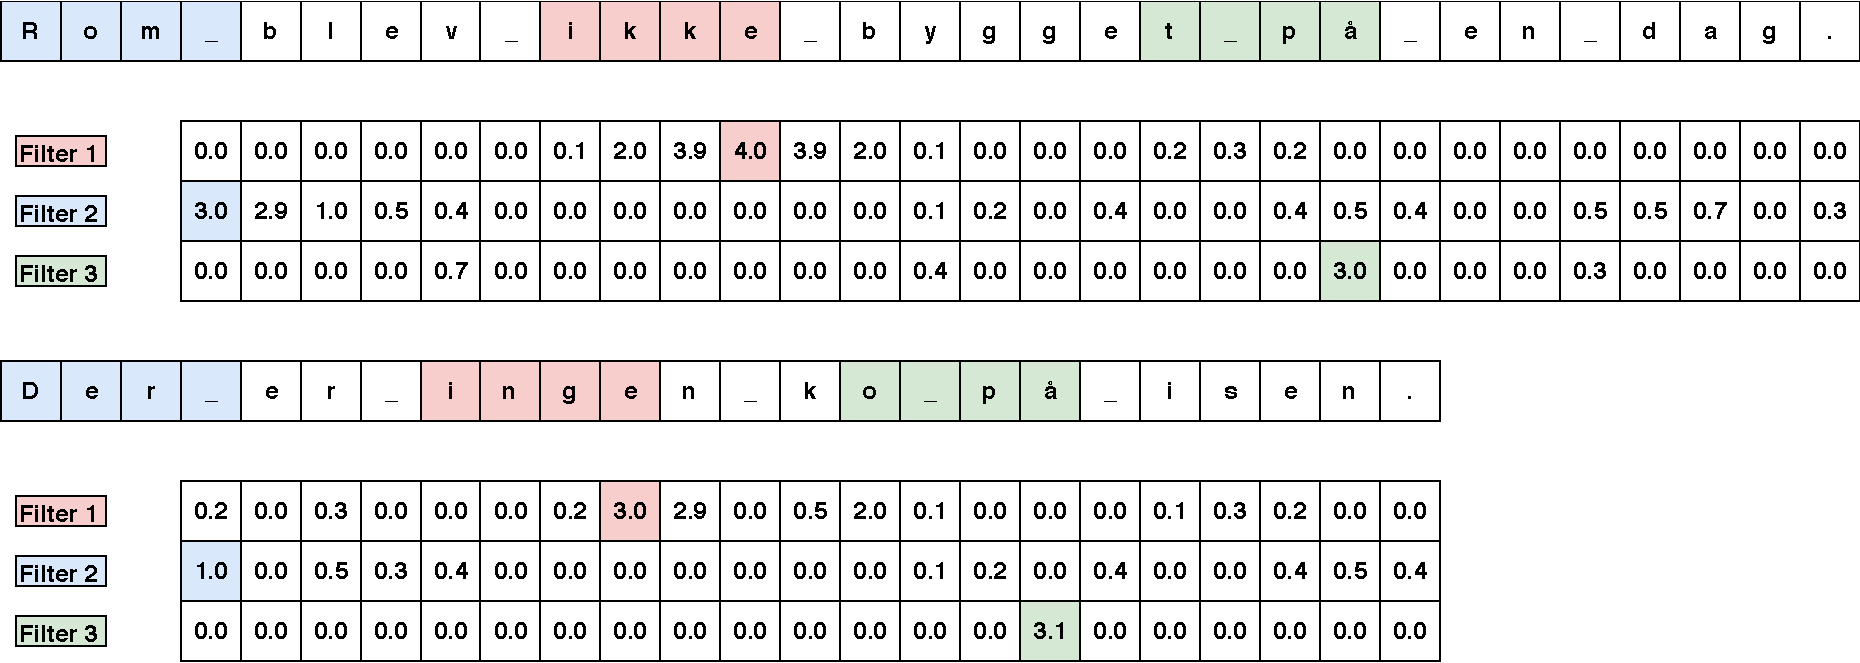
\includegraphics[width=\textwidth]{./pictures/discussion/teacher_feedback_example}
    \caption{Illustrates our feedback to teachers. The particular network
    used in this example only has three filters. The three filters' maximum
    activations are shown in three different colors for the two texts they are
    comparing. The first filter looks for negative qualifiers. Therefore, it
    reacts strongly to both the Danish word "ikke" (not) and part of the Danish
    word "ingen" (none). The second filter looks for city names and reacts
    strongly to the string "Rom " (Rome) but less strongly to "Der " (not a city
    name) even though it looks like a city name. The third filter reacts to
    phrases that contains the word "p\aa " (on) and therefore reacts equally to
    both texts}
    \label{fig:feature_extraction_output_example}
\end{figure}

It is hard to know exactly what the following layers do with the absolute
difference, but we hypothesize that it is a fair assumption that the largest
filter differences translate to the most important differences. The feedback
system we implemented for teachers takes an author $\alpha$, text $t$ and $n
\in \mathbb{N}^+$ and outputs the $n$ largest differences between each $t' \in
T_\alpha$ and $t$. The idea is that when our system reports a negative, the
teacher can ask for feedback from the system. The teacher will then receive a
list of the $n$ greatest differences between each of the texts and can use that
information to strengthen the claim that a student used a ghostwriter.

As an example, we ran our system on a random author and a text 
that author did not write. The whole output can be seen in Appendix
\ref{subsec:teacher_feedback_text_comparisons}. We have shown a truncated
output in Table \ref{tab:teacher_feedback_output}. The output contains only
the comparison between one of the candidate authors' texts and the unknown
text. Text 1 is from the candidate author and Text 2 is the unknown text. 
The three substrings that generated the highest values on dataset \gls{C}
are used to illustrate what each of the filters are looking at.

\begin{table}
    \begin{tabular}{lll|lll}
        \textbf{Max 1}    & \textbf{Max 2}    & \textbf{Max 3}       &
        \textbf{Text 1}   & \textbf{Text 2}   & \textbf{Difference}  \\
        \hline
        \verb[nemlig 1[   & \verb[nemlig 1[   & \verb[nemlig –[      &
        \verb'pere.\n\nH' & \verb'nemlig b'   & |3.06 - 4.70| = 1.64 \\

        \verb[, F.eks.[   & \verb[, F.eks.[   & \verb[, F.eks.[      &
        \verb'. F.eks.'   & \verb'del. Und'   & |4.73 - 3.18| = 1.55 \\

        \verb[ke …''. [   & \verb[a...''\n\n[ & \verb[n''. '' [      &
        \verb'v. Men d'   & \verb'n. Den v'   & |4.28 - 2.91| = 1.37 \\

        \verb[forsøger[   & \verb[forsøger[   & \verb[forsøger[      &
        \verb'for sætt'   & \verb'forsøgte'   & |3.40 - 4.77| = 1.37 \\

        \verb[, Hvorda[   & \verb[, Hvorda[   & \verb[,08 – 6,[      &
        \verb', som ti'   & \verb', Hvorda'   & |3.70 - 5.07| = 1.37 \\

        \verb[der; ’’M[   & \verb[der; ”Ha[   & \verb[der; ”Ma[      &
        \verb'dem; Nia'   & \verb'der omha'   & |4.64 - 3.28| = 1.36 \\

        \verb[. Her ef[   & \verb[. Her ef[   & \verb[' Her br[      &
        \verb'. Jeg vi'   & \verb'. Her fo'   & |2.61 - 3.92| = 1.31 \\

        \verb[r dog kr[   & \verb[r dog kr[   & \verb[r dog ’d[      &
        \verb'r og lud'   & \verb'r dog i '   & |2.83 - 4.13| = 1.30 \\

        \verb[11], da [   & \verb[:1], da [   & \verb[:1], da [      &
        \verb'ys”, der'   & \verb'for, da '   & |3.78 - 5.04| = 1.26 \\

        \verb[, så Car[   & \verb[, så Car[   & \verb[, så Car[      &
        \verb', så er '   & \verb', som En'   & |5.19 - 3.94| = 1.25 \\
        \hline
        \verb[; ’S[       & \verb[; ’S[       & \verb[; ’E[          &
        \verb'; Ni'       & \verb'r He'       & |3.12 - 1.78| = 1.34 \\

        \verb[; ”t[       & \verb[; ”t[       & \verb[; ”t[          &
        \verb'; ”H'       & \verb', ”j'       & |3.44 - 2.13| = 1.31 \\

        \verb[d.’ [       & \verb[d.’ [       & \verb[d.’ [          &
        \verb'ne-V'       & \verb'20’e'       & |1.75 - 2.77| = 1.02 \\

        \verb[1\n’’[      & \verb[1]’’[       & \verb[1]’’[          &
        \verb' l2-'       & \verb'720’'       & |1.75 - 2.71| = 0.96 \\

        \verb['Det[       & \verb['Det[       & \verb['Det[          &
        \verb'ndet'       & \verb' Det'       & |2.37 - 3.25| = 0.88 \\

        \verb[f 1"[       & \verb[f 1"[       & \verb[f 1"[          &
        \verb'f 2\n'      & \verb'v og'       & |3.05 - 2.20| = 0.85 \\

        \verb[æk''[       & \verb[’’ é[       & \verb[ud;'[          &
        \verb'lv; '       & \verb',tro'       & |2.60 - 1.77| = 0.83 \\

        \verb[\n\nx\n[    & \verb[\n\nx\n[    & \verb[\n\nx\n[       &
        \verb'\n\n\n\n'   & \verb'\n\n5\n'    & |1.81 - 2.61| = 0.80 \\
        \verb[ “… [       & \verb[ “… [       & \verb[?“! [          &
        \verb'nd” '       & \verb'r,” '       & |1.75 - 2.53| = 0.78 \\

        \verb[S\n, [      & \verb[S\n, [      & \verb[O\n, [         &
        \verb'e\n, '      & \verb'ad, '       & |2.62 - 1.92| = 0.70 \\
    \end{tabular}

    \caption{Shows the 10 most different activations of convolutional filters
    on two different texts. Both the 10 most different activations for the
    filters of size 8 and size 4 are shown. What each filter is looking at is
    represented by the three greatest activations on any text in the \gls{C}
    dataset. The strings the filter reacted most strongly to are shown in column
    \textbf{Text 1} and column \textbf{Text 2}. The actual activation values
    are shown in the column \textbf{Difference} where the left number corresponds
    to text 1 and the right to text 2. The filters are sorted so the
    greatest difference activation is at the top and the differences fall as we
    move down the list.}

    \label{tab:teacher_feedback_output}
\end{table}

Some of the filters are very clear about what they look at while others require
some parsing. One of the easier filters considers the filter activating to the
string "F. eks". That phrase is Danish for "for example" or "for instance" and
some people write that as "for eksempel" while others use the shorthand above.
If this suddenly changes it could indicate that you are not the author of an
assignment. That cannot be the only reason given, but if thousands of those
reasons are present you can say with some confidence that someone else has
written the assignment. As an example of one of the harder to parse filters
consider the filter looking at \verb["ke …''."[, \verb["a...''\n\n"[ and
\verb["n''. '' "[. That filter seems to react to non-alphanumeric characters,
but on the two texts we are comparing none of the reactions look anything like
what gives the highest numbers. Instead the filter seems to also pick up on the
start of sentences.


\subsubsection{Locating Ghostwritten Areas}
\label{subsubsec:ghost_written_areas}

Aside from feedback based on an entire text, we looked at whether or not we
could say something about which parts of an assignment are the most likely to be
ghostwritten. That would allow a suspicious teachers to identify the part of
the assignment which is least likely to be written by the student and further
analyze that small subsection of the assignment. To find the parts of a text
$t$ most likely to be ghostwritten we split $t$ into a list of paragraphs.
Each paragraph is separated by at least 2 newline characters. We throw away
paragraphs of less than 100 characters since it does not make sense to predict
on such a small amount of text. Hereafter we use one of our networks to compare
each individual paragraph against all of the author's other texts. We take the
average of the comparisons and can then report which paragraphs in the file are
least similar to the author's other texts.

To see how well that system worked we looped through each $\alpha \in
\mathcal{A}$ where $\mathcal{A}$ is the \gls{C} dataset. For each $\alpha$ we
chose a random text $t$ with more than 5 paragraphs. We then split that text up
into paragraphs and removed all paragraphs except the first 5. We then chose
a text $t' \not\in T_\alpha$ and chose a random paragraph from that text. We
then used \gls{conv-char-NN} to predict the 5 paragraphs from $t$ and single
paragraph from $t'$ against each $t'' \in T_\alpha \setminus \{t\}$. We computed
the average prediction on each of the 5 first paragraphs in $t$ and the average
prediction on the paragraph from $t'$. We expect that the average prediction on
paragraphs from $t$ is higher than the paragraph from $t'$.

The predictions on the 5 paragraphs from $t$ was 0.42216, 0.43975, 0.44447,
0.44543 and 0.44425 while the prediction on the paragraph from $t'$ was 0.39524.
As expected we see that the paragraph from text $t'$ has a lower average score
than the 5 paragraphs from $t$. The difference is not as large as we would
have expected however. It seems as if the difference is small enough that
we cannot rely on the results when used on a single assignment. It is also
interesting that no predictions have above 50\% chance of being written by
$\alpha$. It seems like our network does not work well on texts as short as
a single paragraph. That makes sense since the network works by extracting
information from 1200 global max pools and comparing the output from two texts.
Short texts will not be able to achieve an activation of a enough of the filters
for it to be similar to a longer text. The character limit we chose in this
experiment was 100 characters while it was 400 when we trained the networks
which might also be part of the reason.

It is also interesting that the first two paragraphs from $t$ received a lower
average score than the last 3. It seems like the network is better at predicting
the middle of a text than the start of a text.

Another usage for the single paragraph predictions could be for classification
of group assignments. By using the prediction of each paragraph against the
collaborators behind the assignment. It could also be used to detect what amount
of a group assignment was written by what member of said group.


\subsubsection{Applying Other Machine Learning Methods}

We have also considered using other machine learning methods to give feedback
to teachers. Simpler machine learning models has the advantage that it is much
easier to interpret their results compared with neural networks. Consider for
example logistic regression as described by \citet{Abu-Mostafa:2012:LD:2207825}.
The input to the logistic regression is a vector of features and the output is a
probability,

\begin{equation}
    h(\mathbf{x}) = \theta(\mathbf{w}^Tx)
\end{equation}

where $\mathbf{w}$ is the weights of the model and $\theta$ is the sigmoid
function. Here the importance of each individual feature is easily
found as it can be read directly from the weights vector. The downside
to logistic regression models is that they are "only" linear models
\citep{Abu-Mostafa:2012:LD:2207825}. They are therefore not able to model
arbitrary functions. But we could still apply logistic regression to the output
of the feature extraction layer. If we did that we could get an idea of which
features are the most important extracted by the network. We could then use
that information to report to teachers which of the filters they should be most
attentive of.

In a previous project \citep{US} we used the random forest method in an
authorship verification task. The random forest has a build in notion of feature
importance as it relates to the number of times trees split on a particular
feature. Random forests are not normally applied to raw data as we do with our
networks but to a set of features like logistic regression or our baseline
methods. Again it is much easier to get information from a random forest about
which features are the most important and furthermore the forest is able to
model non-linear data. We could therefore also try applying a random forest to
the features extracted by the neural network. Alternately the random forest
model could be applied using a separate set of features. A neural network would
perform the prediction, and in the negative cases a random forest model would
be trained with the purpose of pointing towards the cause. From that we would
be able to conclude which features are the most important for this authorship
verification task.


\subsection{Applicability of Method}\label{subsec:applicability_of_method}

In this section we will discuss how applicable our approach will be to real
world situations. We have created our solutions in a lab setting which
simplifies the problem quite a bit. We discuss here how our results can be
applied to find real ghostwriters.


\subsubsection{Data Deficiencies}

The biggest problem with our approach is that we had no actual ghostwritten
assignments available. We were given a dataset of students where each student
had written a set of assignments. To create ghostwritten assignments we
used assignments turned in by other students. It would of course have been
better if we had had a dataset of students where each student had a set of
assignments known to be written by him/her and a set of assignments known to
have been written by a ghostwriter hired by that student. That was not possible
however since MaCom did not have that data. In a real ghostwriter setting the
ghostwriter might try to mimic the writing style of a student and in that way
might trick our algorithm into classifying a \gls{FP}.

We have discussed another problem with our dataset during the experiments we
performed. We observed multiple times that the network were reacting strongly
to strings looking like Danish names and school class identifiers. On our
artificially constructed dataset all of an authors texts will have the correct
name and most generated ghostwritten texts will have a different name.
Therefore names are an excellent feature to look at due to the way our dataset
was constructed. In a real ghostwriter setting however the names attached to an
assignment is a useless feature as a ghostwriter will always put the students
name on the assignment. We have tried to work against these deficiencies of
our dataset by removing as many names as possible and as much other metadata
information as possible.

We know that we removed a significant amount of information from the texts since
we observed the training and validation accuracy falling after the change. We
also saw less of the filters looking at text metadata suggesting that it is not
as important to the networks.

It is hard to predict exactly how well the network will perform on ghostwritten
assignments when we had no such assignments available during testing. However we
believe we have handled the deficiencies in the dataset as well as possible.


\subsubsection{Applicability to non Danish Class Texts}

The assignments provided to us for the development of this paper was texts
from the Danish course. Therefore the models almost certainly fitted features
that are specific to texts from that course. Thus a certain bias towards the
specific course is to be expected. It would stand to reason, that assignments
made in the Danish course are more focused on the higher linguistic levels such
as \gls{POS}-tags and words. Meanwhile courses such as Maths would focus more
on the individual characters used such as "=", "?" and numbers. One could take
this even further and apply similar methods to code, which suddenly introduces a
lot of formatting specific quirks. Thus the applicability of our current methods
has a bias towards texts from the Danish course and maybe even the specific
skill level of a secondary school student. Students at that age might very well
have a general tendency towards some specific writing style that students on a
higher level does not. That could result in specific network design decision
working better on one group than another. In order to verify how generalizing
our methods are further experimentation into these areas would be needed.

However we believe that if we trained the same networks on data from other
courses we could obtain a model that had comparable performance to the models
trained in this thesis. The model would probably find other n-grams to extract
from the texts but the same architecture would probably still give about similar
results.


\subsubsection{Intentional Cheating of System}

Assuming that a student had obtained information about the inner working of
the system would he/she be able to cheat the system? Cheating would be if
the student did not write an assignment him/herself but still had the text
classified as written by him/her. In a previous section we described how we
can figure out what the convolutional networks is looking at by looking at
the output of the filter extraction layer. If a student could obtain that
information she could make sure that any ghostwritten assignments contained the
same phrases that the network reacted to each time. It would however be very
hard to make sure that all filters received the same values in a ghost written
assignment. The student would have to go through the ghostwritten assignment and
making sure that each filter is represented by approximately the same phrase as
he/she usually use in an assignment. And even if the student obtains the correct
values for most filters the few filters that obtained a different value might be
very important in the dense layers that followed the feature extraction layers.
It is very hard to predict what the dense layers are doing with the features it
is given so it is in our opinion impractical to cheat the convolutional networks
by engineering the features in a ghostwritten assignment.

The problem is even harder in our \gls{RNN} networks. Here the student has even
less information available since it is not possible to tie the reaction of the
\gls{RNN} to particular places in a text.

What the student could do is exploit our prediction system. Some of the
prediction systems we have discussed is especially easy to cheat. Lets for
example consider the $P_{max}$ prediction system. In this prediction system a
text would have to be similar to only a single other text to be considered not
ghostwritten. A student could therefore seed his ``library'' of texts by buying
a ghostwritten assignment for a not very important assignment. That would
probably not result in a problem since teachers will not be as on guard when
it is only a small assignment. Then when they turn in their \gls{SRP} they can
use the same ghostwriter with no problem since they have seeded one of his/her
texts into their library.


\subsubsection{Scalability}

Scalability of the system is important if it is to be implemented. It has to be
possible to apply our methods to all turned in assignments in the system. As
described in an earlier section we chose to implement generalizing models as
they only have to be trained once. The training time is clearly the most costly
part of our implemented methods. The networks take several days to train on
the dataset we currently have and in the future the models might be trained on
even more data increasing the training time further. However when the network
is already trained it can be used an arbitrary number of times to classify
new assignments. The networks might need retraining once in a while to keep
up with general writing style changes over all students. To see why that is
needed consider the filter looking at the phrase "F. eks.". Students might
completely stop using that phrase in the future and it will therefore no longer
discriminate between the students.

When the network is already trained the classification time for a single new
assignment is 0.37 seconds for the \gls{conv-char-NN}, 0.16 seconds for the
\gls{rec-sent-NN} and 0.25 seconds for the \gls{conv-char-word-NN}. That is to
compare a new assignment to on average 13 other texts and weighing the results
using the prediction system we need less than half a second on all of our
networks. Furthermore the task is very parallelizable. An unbounded number of
machines can be set up with a copy of the network and classify new assignments.
The classification time experiment were performed on a cheap laptop so it can
probably also be reduced substantially on a better machine.

For comparison \citet{hansen2014} found that using their author specific
\gls{SVM} model took 0.78 seconds when restricting each student to 5 assignments
and 5.4 seconds when using 16 assignments. That is at least twice as long as
our classification time. \citet{hansen2014} notes that in 2012 roughly 47.000
students finished their final Danish exam assignments at the same time. Using
the 5 most recent assignments \citet{hansen2014} estimated that it would take
$\frac{47,000 \cdot 0.78}{3600} \approx 10.2$ hours to classify all turned in
assignments. Using our methods the same computation would take $\frac{47,000
\cdot 0.37}{3600} \approx 4.8$ hours for the \gls{conv-char-NN}, $\frac{47,000
\cdot 0.16}{3600} \approx 2.1$ hours for the \gls{rec-sent-NN} and $\frac{47,000
\cdot 0.25}{3600} \approx 3.3$ hours for the \gls{conv-char-word-NN}.

The average classification time of our methods could potentially be reduced
further by trading memory usage for runtime. The statistics we have presented in
this section is based on the classification time when predicting only a single
pair of texts at a time. However the network is able to predict an arbitrary
number of pairs at a time. Instead of predicting each pair independently batches
of $n$ comparisons could be set up in a matrix and predicted at the same time
reducing the runtime substantially. The networks use highly optimized matrix
libraries for the classification and if performed on a graphics card which is
optimized for such operations it could be very fast.


\subsubsection{Citations}

Citations are a problem for our networks since an authors writing style will be
poluted by a different authors writing style. Depending on which course the text
is in the amount of citations will differ. A course with a hefty focus on third
party sources such as history will most likely have an increase in citation
usage. This is not something our models compensate for. Citations introduce a
break in the linguistic patterns exhibited by the student. For this reason each
citation serves as a source of noise for our models. The solution for this is
simple and will be addressed in Section \ref{sec:future_work}. There is however
another citation problem which is not easily addressed. A student could perform
some direct copying of external sources, without marking it as such. This would
give the same break in linguistic patterns, but would not be nearly as easily
detectable. MaCom already have systems in place for detecting plagiarism when
copied from the internet. Assignments given to our system should first be
checked for plagiarism to prevent our system from learning from plagiarised
texts. It should be noted that there would be cases where citation would add to
the accuracy of the model. This would be cases where a student for some reason
uses the same sources consistently for their assignments. In this scenario we
suspect our models would perceive the contents of the citations as part of the
student vocabulary.


\subsubsection{Group Handin}\label{subsubsec:group_handin}

There is also the scenario where rather than a single student handing in an
assignment. For example a collaborative assignment between several students.
In this scenario writing style would not be consistent throughout the paper,
seemingly rendering our methods useless. If our methods were to work right
out of the box, the work of a group of students would have to be represented
in the training data, as if they were a single student. In this scenario our
methods ideally would learn how they wrote as a group. This scenario is however
very unlikely to happen. It presupposes that students only operate in the same
groups throughout their years in high school. Not only that, but in order to
train our methods, a substantial portion of the students would have to do this.
For this reason the above described scenario most likely would not apply in
practice. This problem does however have a solution, which is described in
Section \ref{sec:future_work}.


% TODO: Read through section seeing if everything makes sense with fewer graphs
% and a much shortened section with time based weights.
\subsection{Prediction Systems}

As described in Section \ref{subsec:combining_neural_network_output} we
use several weight functions to weight which of an authors texts are most
important. Looking at the graphs in Figure \ref{fig:conv-char-NN-pred-50},
\ref{fig:conv-char-NN-pred-4}, \ref{fig:rec-sent-NN-pred-50},
\ref{fig:rec-sent-NN-pred-4}, \ref{fig:conv-char-word-NN-pred-50} and
\ref{fig:conv-char-word-NN-pred-4} we can get an idea of the relative strengths
of the weight methods. Using those graphs we want to discuss a couple of the
prediction systems.

\begin{description}

    \item[$\mathbf{P_\mathrm{U}}$]

        The uniform prediction system $P_\mathcal{U}$ generally has a lower
        accuracy and higher accusation error than the other prediction systems.
        The only prediction system that performs worse than the uniform weight
        is $P_{min}$. We had expected that the uniform weighing would perform
        worse than the others since it does not use any metadata about the texts
        to make its predictions. It only use the raw predictions on the texts of
        the networks and simply takes an average of that.

    \item[$\mathbf{P_{exp_\lambda}}$]

        The exponential dropoff prediction system used the time of an
        assignment to determine the most important text. Recall that
        as $\lambda \rightarrow \infty$ more weight is placed on the
        newest assignment. We assumed that an authors writing style would
        change over time and the newest text would therefore be a better
        predictor of current writing style than the oldest text. In Figure
        \ref{fig:conv_char_prediction_zoom_50} we have shown a plot of the
        $P_{exp_\lambda}$ and $P_\mathcal{U}$ prediction system accuracies and
        accusation error with important intervals highlighted. The important
        intervals is when $\theta \approx 0$, when $\theta \approx 1$ and when
        the accuracy is maximized around $\theta \approx 0.5$. In both Figures
        we observe that the accuracy is lower and accusation error higher in
        $P_\mathcal{U}$ than all $P_{exp_\lambda}$. We can therefore conclude
        that as expected the newest text is more indicative of the writing style
        of a student than the older texts.

        \begin{figure}
            \centering
            \textbf{$\mathbf{P_{exp_\lambda}}$ 50\% Negative Samples}\par\medskip
            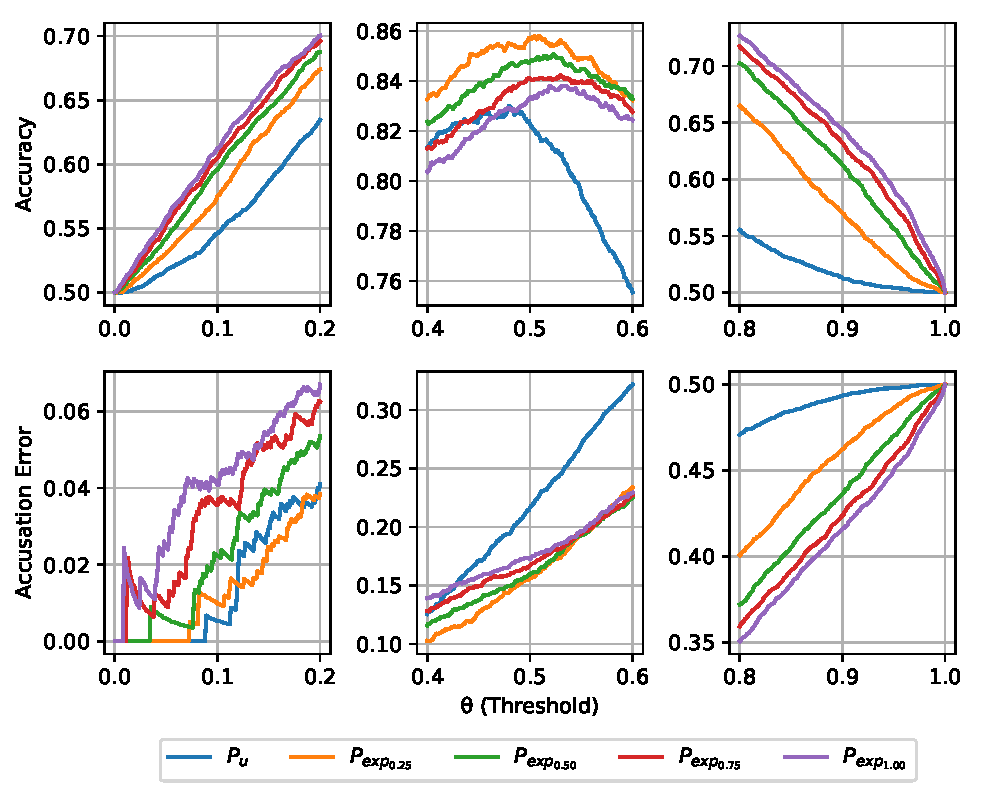
\includegraphics[width=0.7\textwidth]{./pictures/discussion/conv_char_nn_prediction_zoom_50_time}
            \caption{Illustrate important intervals for our different
                $P_{exp_\lambda}$ prediction systems for the \gls{conv-char-NN}
                network on the dataset with 50\% negative samples. On the left
                we have shown the beginning of the curves, in the middle we have
                shown the top accuracy and to the right we have shown the end of
                the curves.}
            \label{fig:conv_char_prediction_zoom_50}
        \end{figure}

    \item[$\mathbf{P_l}$]

        The idea behind the length based prediction system was that
        longer texts would better reflect the writing style of an
        author. Some of the texts in the dataset are only a few hundred
        characters long which means that only few of the n-grams the
        networks are looking for will be present in those texts. In Figure
        \ref{fig:conv_char_prediction_zoom_50_text_length} we have shown a
        comparison between $P_\mathcal{U}$ and $P_l$. It can be seen there that
        it is always better to weight based on text length than it is to just
        use uniform weights. The curves follow each other closely but $P_l$
        have slightly higher accuracy and slightly lower accusation error than
        $P_\mathcal{U}$. That is exactly the result we expected and shows that
        it was a good idea to look at text length as part of our prediction
        systems.

        \begin{figure}
            \centering
            \textbf{$\mathbf{P_l}$ \& $\mathbf{P_{lexp_{0.25}}}$ \&
            $\mathbf{P_{exp_{0.25}}}$ 0.5 Split}\par\medskip
            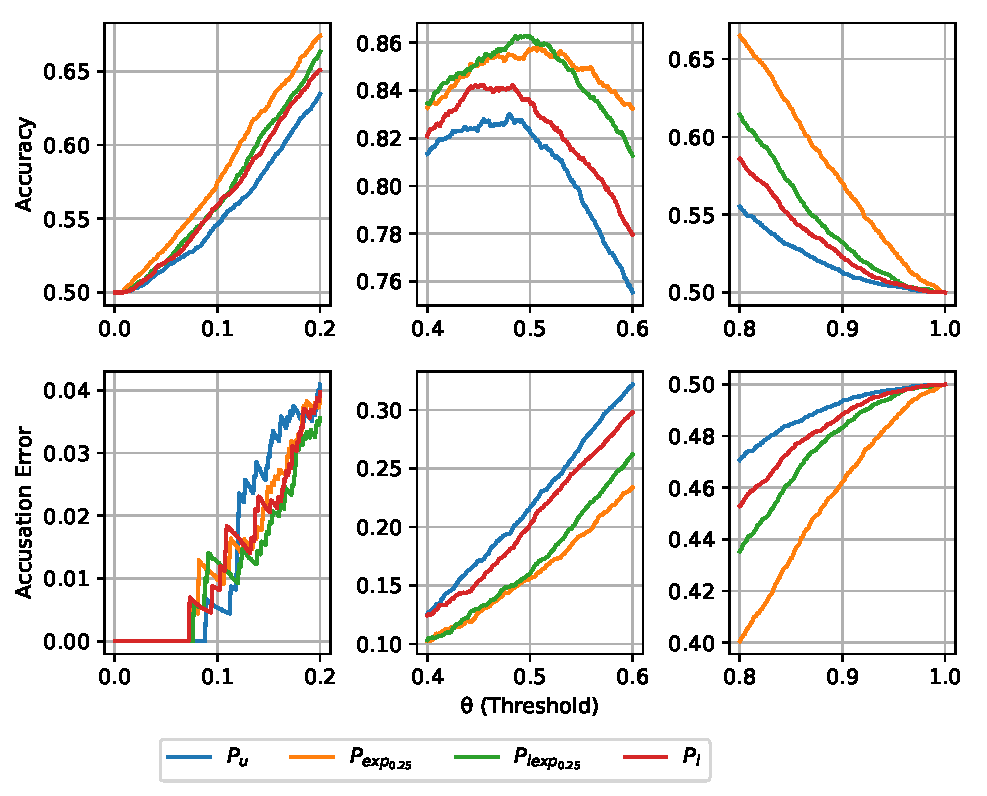
\includegraphics[width=0.7\textwidth]{./pictures/discussion/conv_char_nn_prediction_zoom_length}
            \caption{Illustrate important intervals for our $P_l$,
                $P_{exp_\lambda}$ and $P_{lexp_{\lambda}}$ prediction systems
                for the \gls{conv-char-NN} network on the 0.5 split dataset. On
                the left we have shown the beginning of the curves, in the
                middle we have shown the top accuracy and to the right we have
                shown the end of the curves.}
            \label{fig:conv_char_prediction_zoom_50_text_length}
        \end{figure}

    \item[$\mathbf{P_{lepx_{0.25}}}$]

        This prediction system were a combination of the time based and text
        length based prediction systems. Multiple different networks had this
        configuration as the configuration that maximized accuracy. We have
        already concluded that both $P_l$ and $P_{exp_\lambda}$ was better
        weightings than $P_\mathcal{U}$. So the interesting thing about this
        weight is not whether or not it beats $P_\mathcal{U}$, but rather
        whether or not it is better than $P_l$ and $P_{exp_\lambda}$. In Figure
        \ref{fig:conv_char_prediction_zoom_50_text_length} we have shown the
        performance of $P_{lexp_\lambda}$.

        In that Figure we see that $P_{exp_{0.25}}$ has generally better
        performance than $P_{lexp_{0.25}}$ except right at the maximum accuracy.
        At the maximum accuracy $P_{lexp_{0.25}}$ is able to just barely beat
        $P_{exp_{0.25}}$. Almost all the networks used the $P_{lexp_{0.25}}$
        prediction system as the best prediction system and it must be this
        small difference that causes that.

        It is interesting that the performance of $P_{lexp_{0.25}}$ is only best
        right at the maximum accuracy. Maybe that is due to something similar to
        the effect we saw with $P_{exp_{\lambda}}$ where higher $\lambda$ values
        was best at the extremes and lower $\lambda$ values were better in the
        middle of the graphs.

    \item[$\mathbf{P_{MV}}$]

        The majority vote prediction $P_{MV}$ system is similar to the
        uniform prediction system $P_{\mathcal{U}}$. We therefore expect
        about similar performance. What can actually be seen in Figure
        \ref{fig:conv_char_prediction_zoom_50_majority_vote} is that in the
        beginning $P_{MV}$ has substantially higher accuracy and accusation
        error. The picture is similar to the $P_{exp_{1.0}}$ prediction system.
        In the middle the uniform weight function is clearly better than the
        majority vote and the accusation error curves cross. At the end of the
        graph the majority vote again has the highest accuracy but now has the
        lowest accusation error. The cause behind this behavior is most likely
        the sane as $P_{exp}$. In the higher and lower ends og $\theta$, more
        a smaller amount of more extreme predictions is needed to get the best
        performance. $P_{MV}$ simply allows for to much negative influence from
        poorly representing texts when using high and low $\theta$ values, much
        like the uniform weighing.

        \begin{figure}
            \centering
            \textbf{$\mathbf{P_{MV}}$ \& $\mathbf{P_{min}}$ \&
            $\mathbf{P_{max}}$ 0.5 Split}\par\medskip
            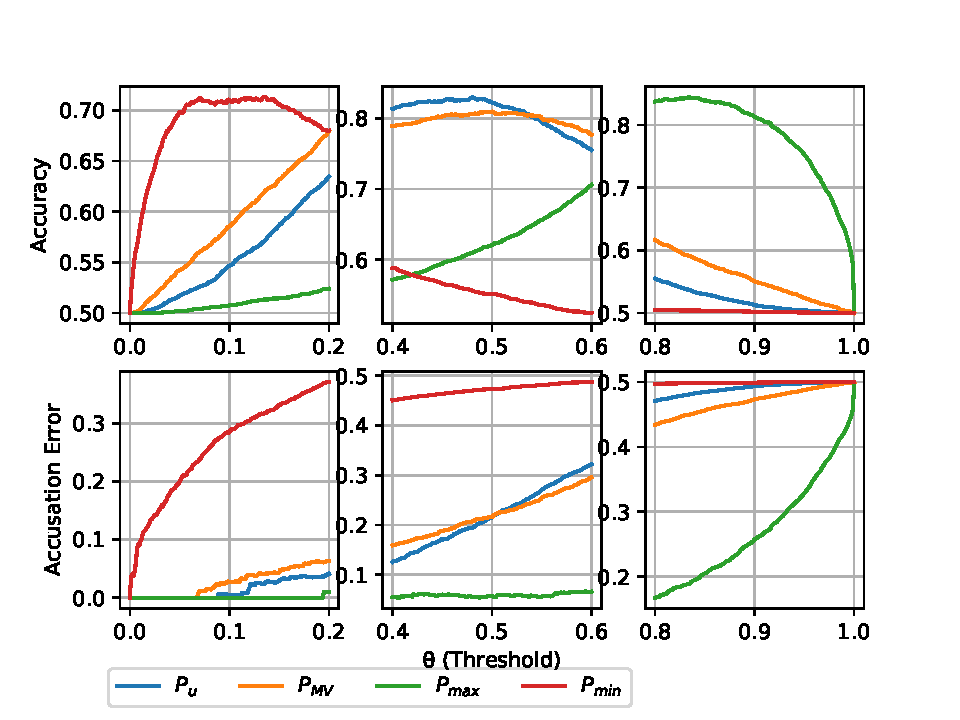
\includegraphics[width=0.7\textwidth]{./pictures/discussion/conv_char_nn_prediction_zoom_min_max}
            \caption{Illustrate important intervals for our $P_{MV}$, $P_{max}$
                and $P_{min}$ prediction systems for the \gls{conv-char-NN}
                network on the 0.5 split dataset. On the left we have shown the
                beginning of the curves, in the middle we have shown the top
                accuracy and to the right we have shown the end of the curves.}
            \label{fig:conv_char_prediction_zoom_50_majority_vote}
        \end{figure}

    \item[$\mathbf{P_{min}}$]

        The $P_{min}$ system is the only prediction system with worse
        performance than the $P_{\mathcal{U}}$ system. The problem is that
        the accusation error rise very quickly. Even though the accuracy
        also rise quickly the accusation error rises so quickly that the
        systems thresholds give to high accusation error to be used. We
        can also see that the maximum accuracy of the $P_{min}$ system
        is around 70\% which is also lower than the other systems. We
        have shown a plot of the $P_{min}$ prediction system in Figure
        \ref{fig:conv_char_prediction_zoom_50_majority_vote}.

    % TODO: Write about P_max

\end{description}


\subsection{Writing Style Changes}
\label{subsec:writing_style_changes}

In this section we discuss how a secondary school students writing style changes
during his/her school years. We observed that time based weights worked well
when doing authorship verification. That suggests that there is some development
in students writing style which would also be expected. Secondary school is
probably one of the time periods writing style changes the most.

To get an idea of how much the writing style of a student changes over time we
looped through each author in the \gls{D} dataset. We created a positive and a
negative sample for each of the authors and used \gls{conv-char-NN} to predict
each of the authors texts against the positive and negative sample. We then
computed the average score of the newest text, the average score of the second
newest text, and so on for both positives and negatives. If the students writing
style changes over time we would expect the newest text having an higher average
score than the oldest texts for the positive samples. We also expect that the
negative samples are to have an average of less then 0.5 but about the same
for each text. In Figure \ref{fig:writing_style_changes} we have illustrated
the average positive and negative predictions produced by our network. We only
predict the newest 20 texts as very few authors in the dataset has more than
that. So the averages of the texts above 20 vary wildly.

\begin{figure}
    \centering
    \textbf{Writing Style Changes}\par\medskip
    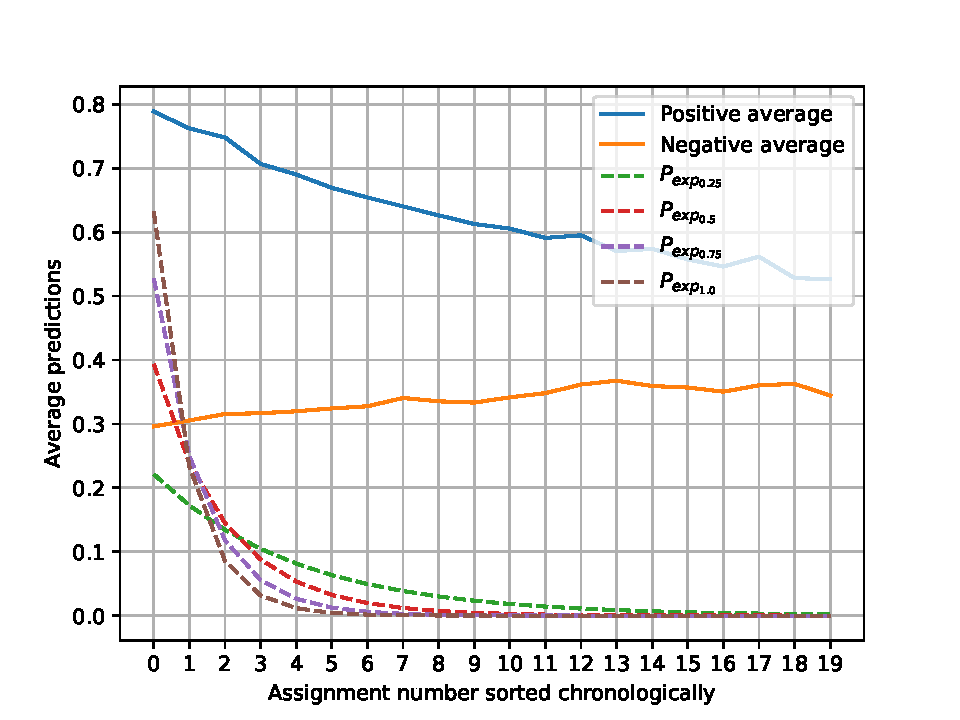
\includegraphics[width=0.7\textwidth]{./pictures/discussion/writing_style_change}
    \caption{Average predictions of newest to oldest texts for positive samples
        and negative samples by \gls{conv-char-NN}. The newest text is shown to
        the left and the oldest to the right. We have also shown a plot of the
        different time based weight functions we tried using.}
    \label{fig:writing_style_changes}
\end{figure}

In that figure it is very clear that writing style does change over time. The
positive samples fall from 80\% prediction on the newest assignment to just
over 50\% on the oldest assignment. That is a very large drop that suggests
that after only 20 turn ins the writing style has changed so drastically that
our network almost believes it is someone else. It is very interesting that the
drop in accuracy seem to follow closely our $P_{exp_{0.25}}$ prediction system
weights. That is probably the reason why that particular $\lambda$ value so
often gave the best results.

The negative curve is a bit weird. We expected it to stay flat below 50\% but
it seems to be rising towards 50\%. The curve is clearly more flat than the
positive curve but there does still seem to be a trend towards 50\%.


% TODO: Add discussion of different filters based on the following filter
% activations. We should discuss why the filters makes sense to look at. It is
% possible to get more filter activations if we need them.
%
% \subsection{Filters}
%
% [', F.eks.' ', F.eks.' ', F.eks.']
% [', mens ’' ', mens ’' ', mens ’']
% [' mandig,' ' mandig,' ' mandig,']
% ['z, og at' 'z, og at' 't, og fx']
% [' \\nSelvom' ' \\nSelvom' '\\n\\nSelvdy']
% ['ag, pga.' 'ag, pga.' '’’, pga.']
% ['om fx ""' 'om fx ""' 'om fx ""']
% ['a. bl,a.' 'm; bl.a.' 'm; bl.a.']
% ['t” dette' 't” dette' 'z, dette']
% ['é, at ha' 'é, at ha' 'é, at ha']
% ['bog; ”Vi' 'tår; ”Ve' 'tos; ”Vi']
% ['r, at ’’' 'r, at ’’' 'r, at ’’']
% ['r dog kr' 'r dog kr' 'r dog ’d']
% ['m hvor d' 'm hvor d' 'm hvad ’']
% [' dum ud,' ' dum ud,' ' dum ud,']
% ['siger: “' 'siger: “' 'siger: “']
% ['Fx. ' 'Fx. ' 'Fx. ']
% ["''Og" "''Og" "''Og"]
% ['Måsk' 'Måsk' 'Måsk']
% ["''.." "'''." '"..d']
